\section{Numerical Results and Discussion}\label{sec:results}

In this section, a realistic case study is considered. All source code is shared in \cite{code}.

\subsection{Load shifting versus mFRR: Which one is more appealing financially?}

We consider five models to calculate the operational (energy) cost of a single freezer, including three models where the freezer provides mFRR services, one model where the freezer shifts the load in response to spot prices, and the last model, the so-called base cost, where the freezer neither shifts the load nor provides mFRR services. The data availability for these five models is summarized in
Table \ref{tab:price_visibility}.




\begin{table}[t]
    \caption{Data availability for each model.}
    \label{tab:price_visibility}
    \centering
    \begin{tabular}{llccc}
        \toprule
        Model         & Curve(s) in Fig. \ref{fig:cumulative_cost_comparison} & $\bm{\lambda}^{\rm{r},\uparrow}$ & $\bm{\lambda}^{\rm{s}}$ & $\bm{\lambda}^{\rm{b}}$ \\
        \midrule
        mFRR oracle   & Dashed black                                          & $\checkmark$                     & $\checkmark$            & $\checkmark$            \\
        mFRR cases    & Blue and red                                          & $\checkmark$                     & $\ast$                  & $\ast$                  \\
        Load shifting & Yellow                                                & N/A                              & $\checkmark$            & N/A                     \\
        Base cost     & Solid black                                           & N/A                              & $\checkmark$            & N/A                     \\
        \bottomrule
        \multicolumn{5}{l}{$\checkmark$: True (realized) data are available.}                                                                                        \\
        \multicolumn{5}{l}{$\ast$: Forecast data (in form of scenarios) are available.}                                                                              \\
        \multicolumn{5}{l}{N/A: Not applicable.}
    \end{tabular}
    \vspace{-2mm}
\end{table}




For these five models, Fig. \ref{fig:cumulative_cost_comparison} shows the out-of-sample cumulative operational cost of the single freezer during the first nine months of 2022. Recall that all these models have been compared fairly by an out-of-sample simulation against identical scenarios, i.e., real spot and balancing market prices from 2022.
The base cost (solid black) has only access to spot price data, and leads to the highest cost in Fig. \ref{fig:cumulative_cost_comparison}.
Blue and red curves (mFRR cases), both below the base cost curve, correspond to the cases where the freezer provides mFRR services, and uses scenarios to model spot and balancing market price uncertainties. Their difference comes from in-sample scenarios used: while the red curve uses five scenarios coming from the most recent historical data (lookback strategy), the blue curve uses 50 scenarios coming from 2021. The yellow curve shows the reduced cost of the freezer due to  load shifting. Finally, the dotted black curve (lowest in Fig. \ref{fig:cumulative_cost_comparison}) provides an oracle (ideal benchmark), where the freezer perfectly knows the spot and balancing market prices.

An interesting observation is that, in comparison to the base cost, load shifting (yellow curve) bring a 13.9\% cost reduction, whereas the mFRR service provision reduces the cost by  11.6\% (red curve) and 10.1\% (blue curve). Note that the cost savings reported for red and blue curves are not far  from the mFRR oracle, showing that the scenarios used are sufficiently good.
While this observation might be appealing to the freezer as load shifting requires a comparatively simpler decision-making process than the mFRR provision, it is not necessarily a desirable outcome for the power system. The mFRR service provision helps the system keep the supply-demand balance, while load shifting as a response to spot prices is not necessarily helping the system, and even in the worse case, the spot prices fixed before load shifting may no longer represent the supply-demand equilibrium. This calls system operators and regulators for potential changes, e.g., market redesign, to make the mFRR service provision more attractable.



\begin{figure}[t]
    \centering
    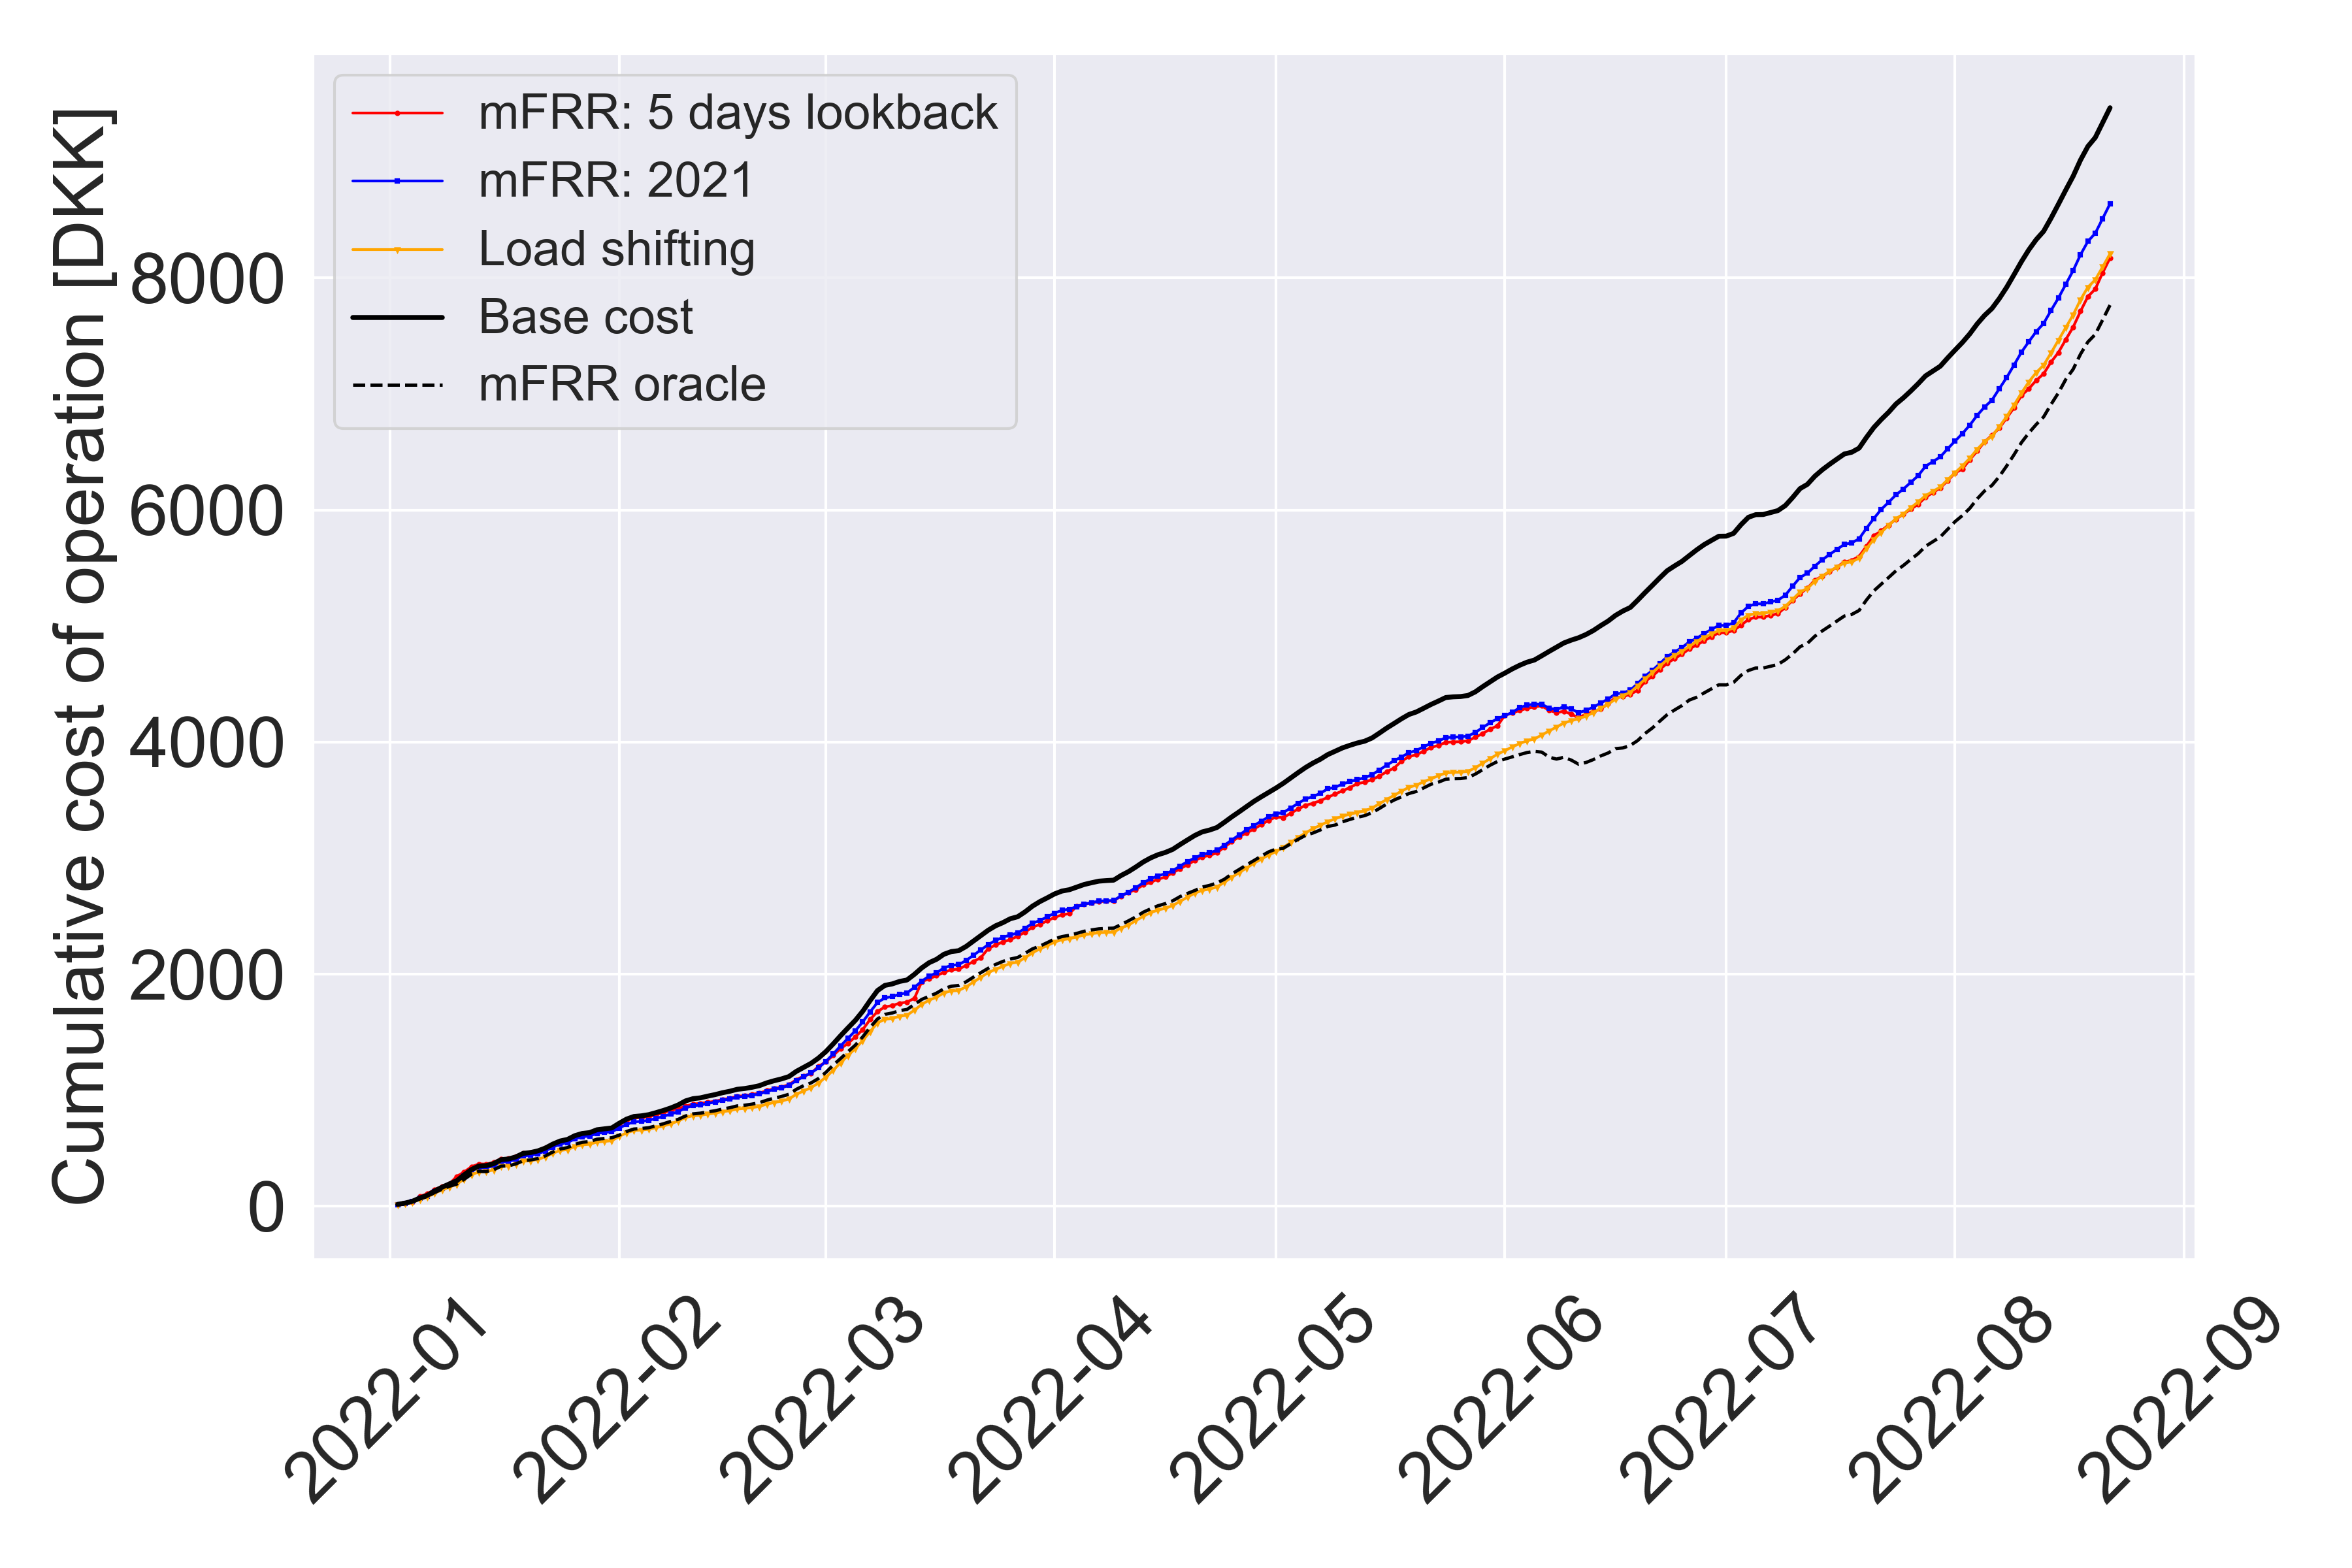
\includegraphics[width=\columnwidth]{../figures/cumulative_cost_comparison.png}
    \caption{Out-of-sample cumulative operational cost for the freezer during the first nine months of 2022.}
    \label{fig:cumulative_cost_comparison}
    \vspace{-2mm}
\end{figure}

In the case of load shifting, it is worth mentioning that the settlement cost of the BRP is ignored --- this reflects the self-interested flexible loads.  While the flexible load reduces her cost by load shifting, the corresponding BRP may incur a settlement cost due to the resulting imbalance between the true consumption and the day-ahead schedule. In practice, the BRP would have to pay for such an imbalance or at least buy/sell energy in the intra-day market to adjust her day-ahead schedule and consider potential load shifting actions by flexible loads. However, loads are not necessarily aware of those costs for the BRP. Hence, they may have a strong incentive to exploit their flexibility for load shifting. Some larger flexible consumers, such as industrial and commercial loads, might not be exposed fully to spot prices, and for those consumers, load shifting could be less profitable. However, they may still have an incentive to change their deal with the BRP to get a full exposure.

In the case of mFRR service provision, it is also  assumed that the entire revenue earned from reservation and activation go to the flexible load. This neglects the fact that, in practice, the BRP requires a share of the revenue. Furthermore, there might be an aggregator or a technology provider who facilitates the aggregation and communication of the flexibility. In such a case, they would also request a share of the revenue. This can potentially reduce the revenue of flexible loads by the mFRR service provision.








%\begin{flushleft}
%    \begin{table}[b]
%        \caption{Average Daily OOS Costs.}
%        \label{tab:cases_compared}
%        \centering
%        \begin{tabular}{lccc}
%            \toprule
%            Name                 & \thead{mFRR w.                   \\lookback} & Load shifting & \thead{mFRR \\w. 2021} \\
%            \midrule
%            Base cost today      & 40.6         & 40.6 & 40.6 \\
%            Total cost           & 35.9         & 35 & 36.5 \\
%            Expected energy cost & 40.6         & 35 & 40.6 \\
%            Rebound cost         & 0.86          & N/A    & 0.9  \\
%            Reserve payment      & 3.2          & 0.0    & 3.4  \\
%            Act payment          & 8.1          & 0.0    & 2.2  \\
%            Penalty cost         & 5.7          & 0.0    & 0.5  \\
%            Scenarios            & -5             & 1      & 50     \\
%            ADMM                 & False          & False  & True   \\
%            \% savings           & 11.6           & 13.9   & 10.1   \\
%            \bottomrule
%        \end{tabular}
%    \end{table}
%            \vspace{-2mm}
%\end{flushleft}


%Table \ref{tab:cases_compared} breaks down the cost components. For mFRR, there is big difference between the lookback strategy and the ADMM strategy with 2021 prices. The lookback strategy earns much more from activation payments, but is also penalized more as it is not able to deliver its reservation capacity in some days. The other mFRR strategy bids more conservatively and is only rarely activated. The market rules prescribe that the full bid should be delivered, hence the lookback strategy might be too risky. On the other hand, it was assumed that the activation power should be equal to the reserved power, but the TSO determines the activation power, hence the activation power might be lower in reality which would both decrease the penalty cost and the activation revenue.

%All strategies are better than the baseline costs, i.e., not utilizing flexibility, with savings of 10-14\%. Furthermore, the mFRR strategies are not far off the theoretically best mFRR strategy as indicated by the oracle in Figure \ref{fig:cumulative_cost_comparison}.


\begin{figure}[t]
    \centering
    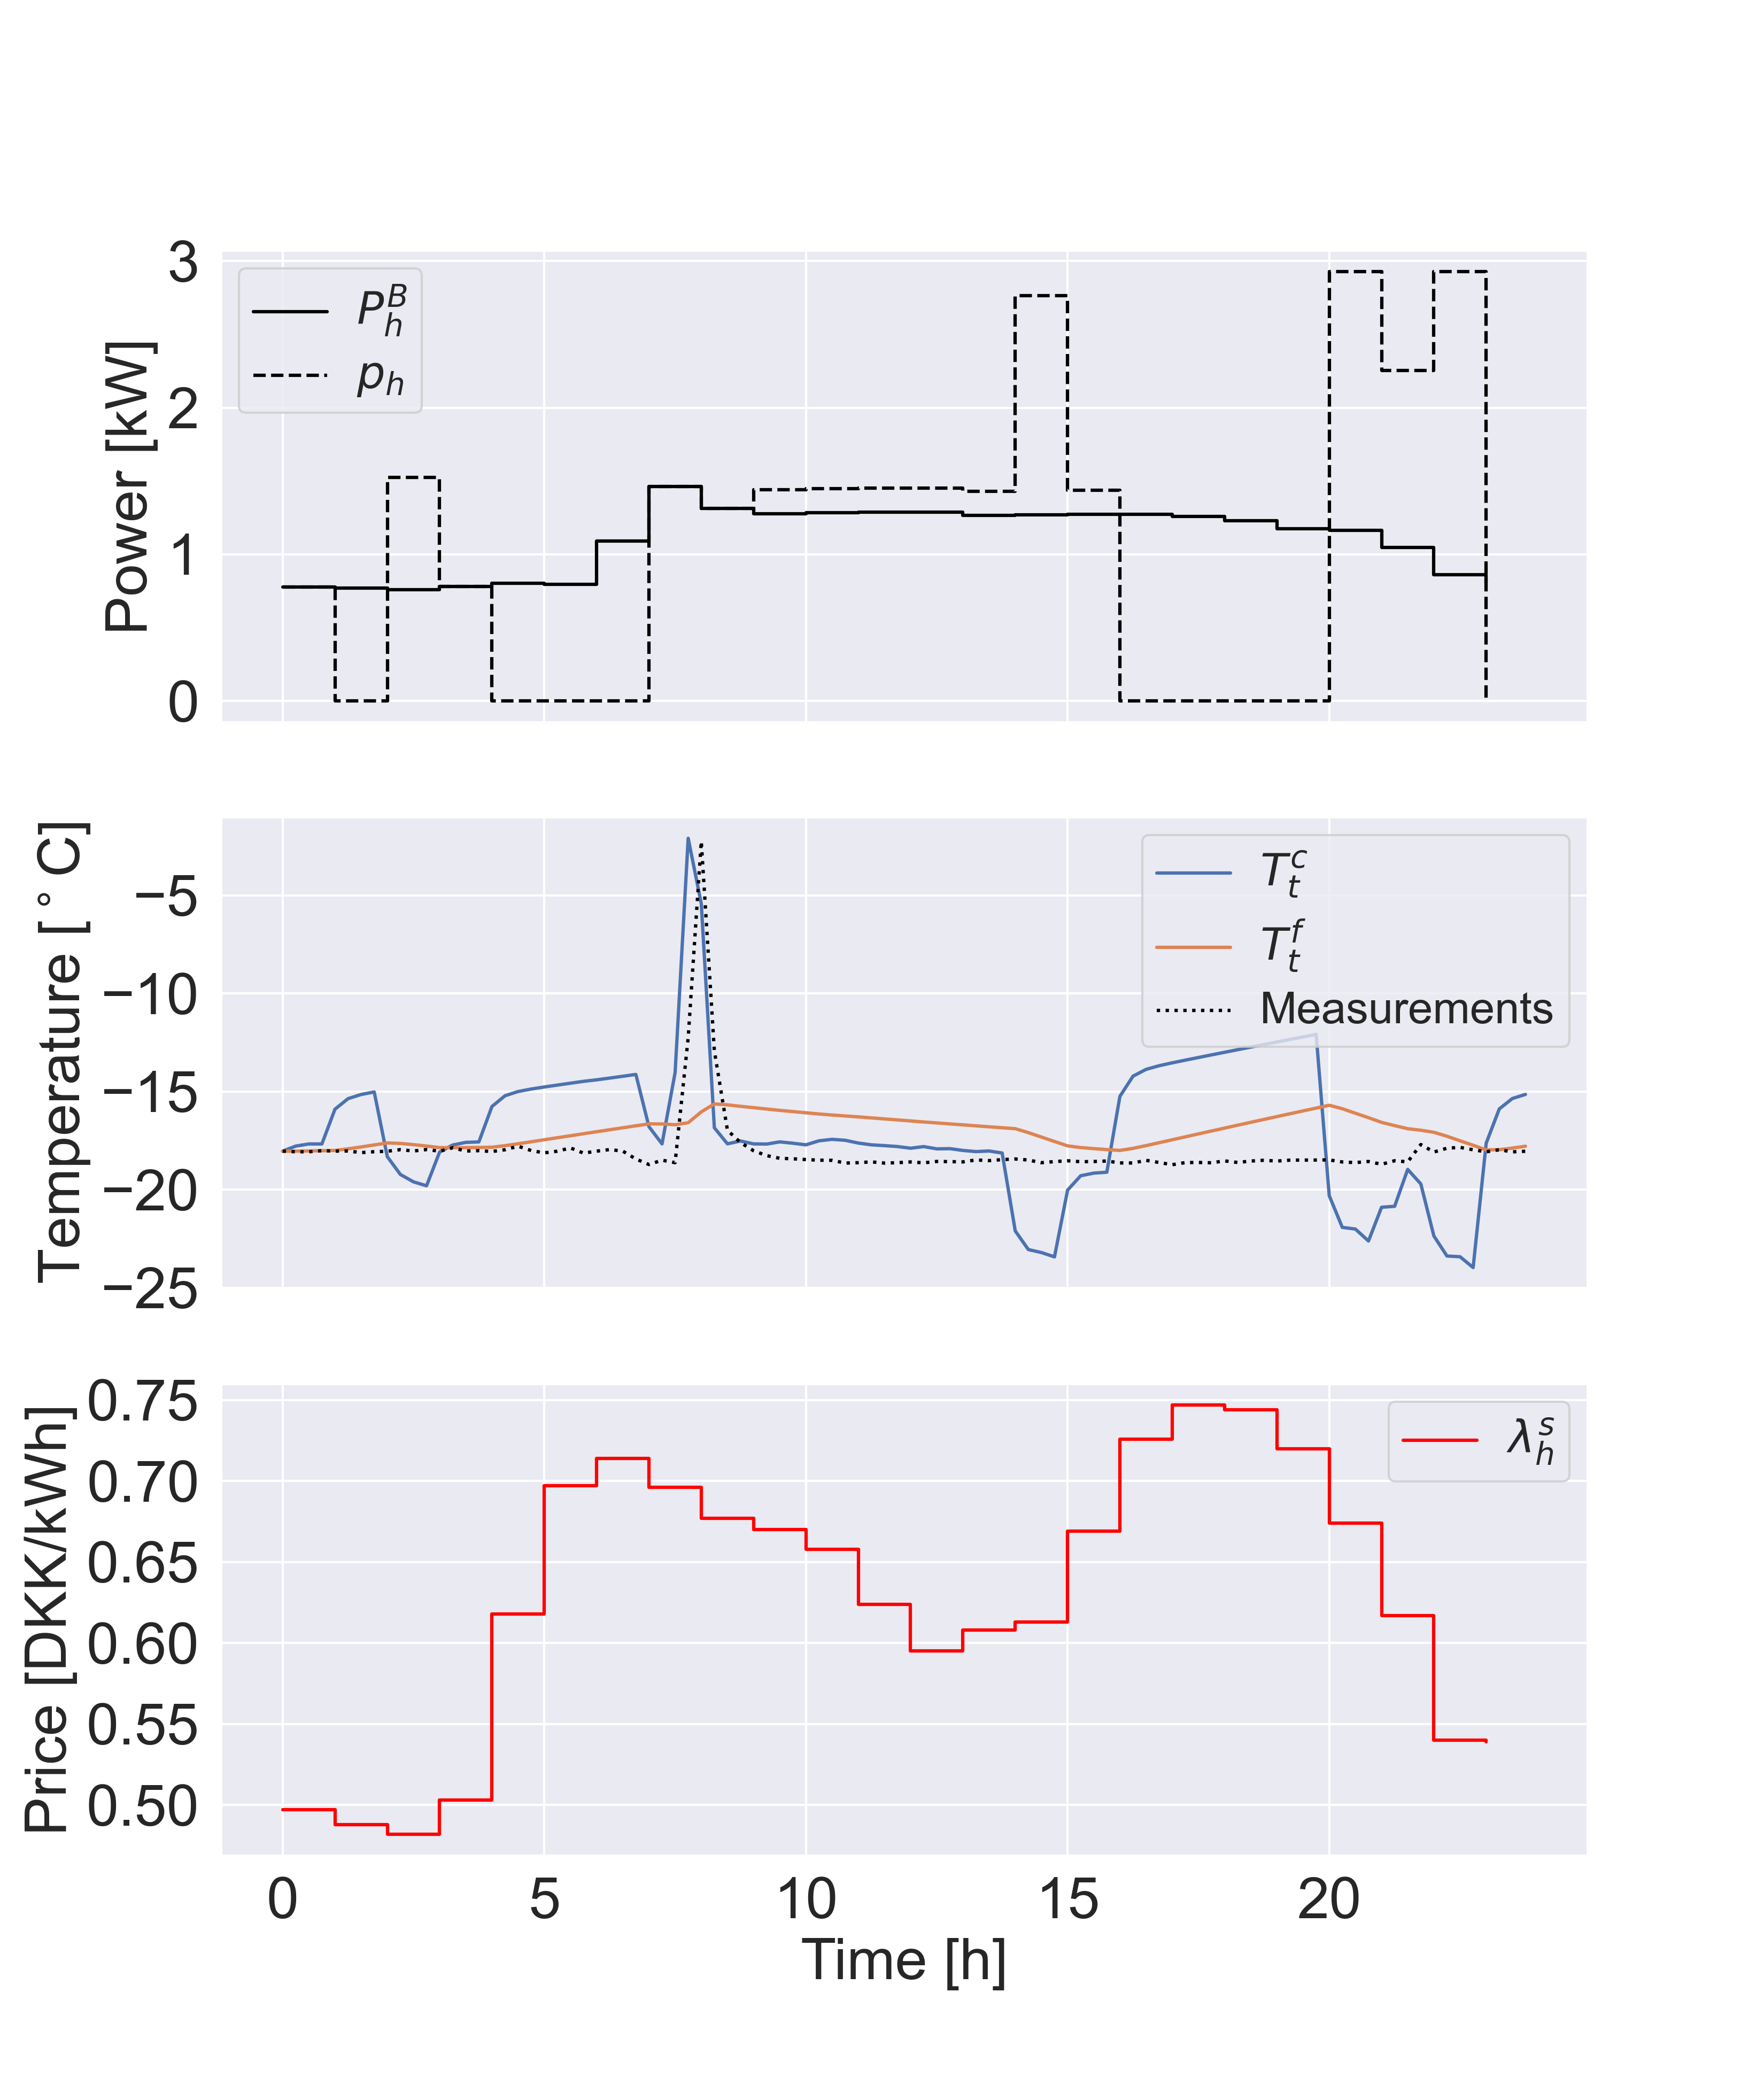
\includegraphics[width=\columnwidth]{../figures/spot_single_case.png}
    \caption{Example of load shifting in a representative day (an in-sample scenario). \textbf{Top}: Baseline consumption of the freezer and the power profile after load shifting. \textbf{Middle}: Air and food temperature dynamics. \textbf{Bottom}: Spot market prices.}
    \label{fig:fig_first_case}
\end{figure}




\begin{figure}[t]
    \centering
    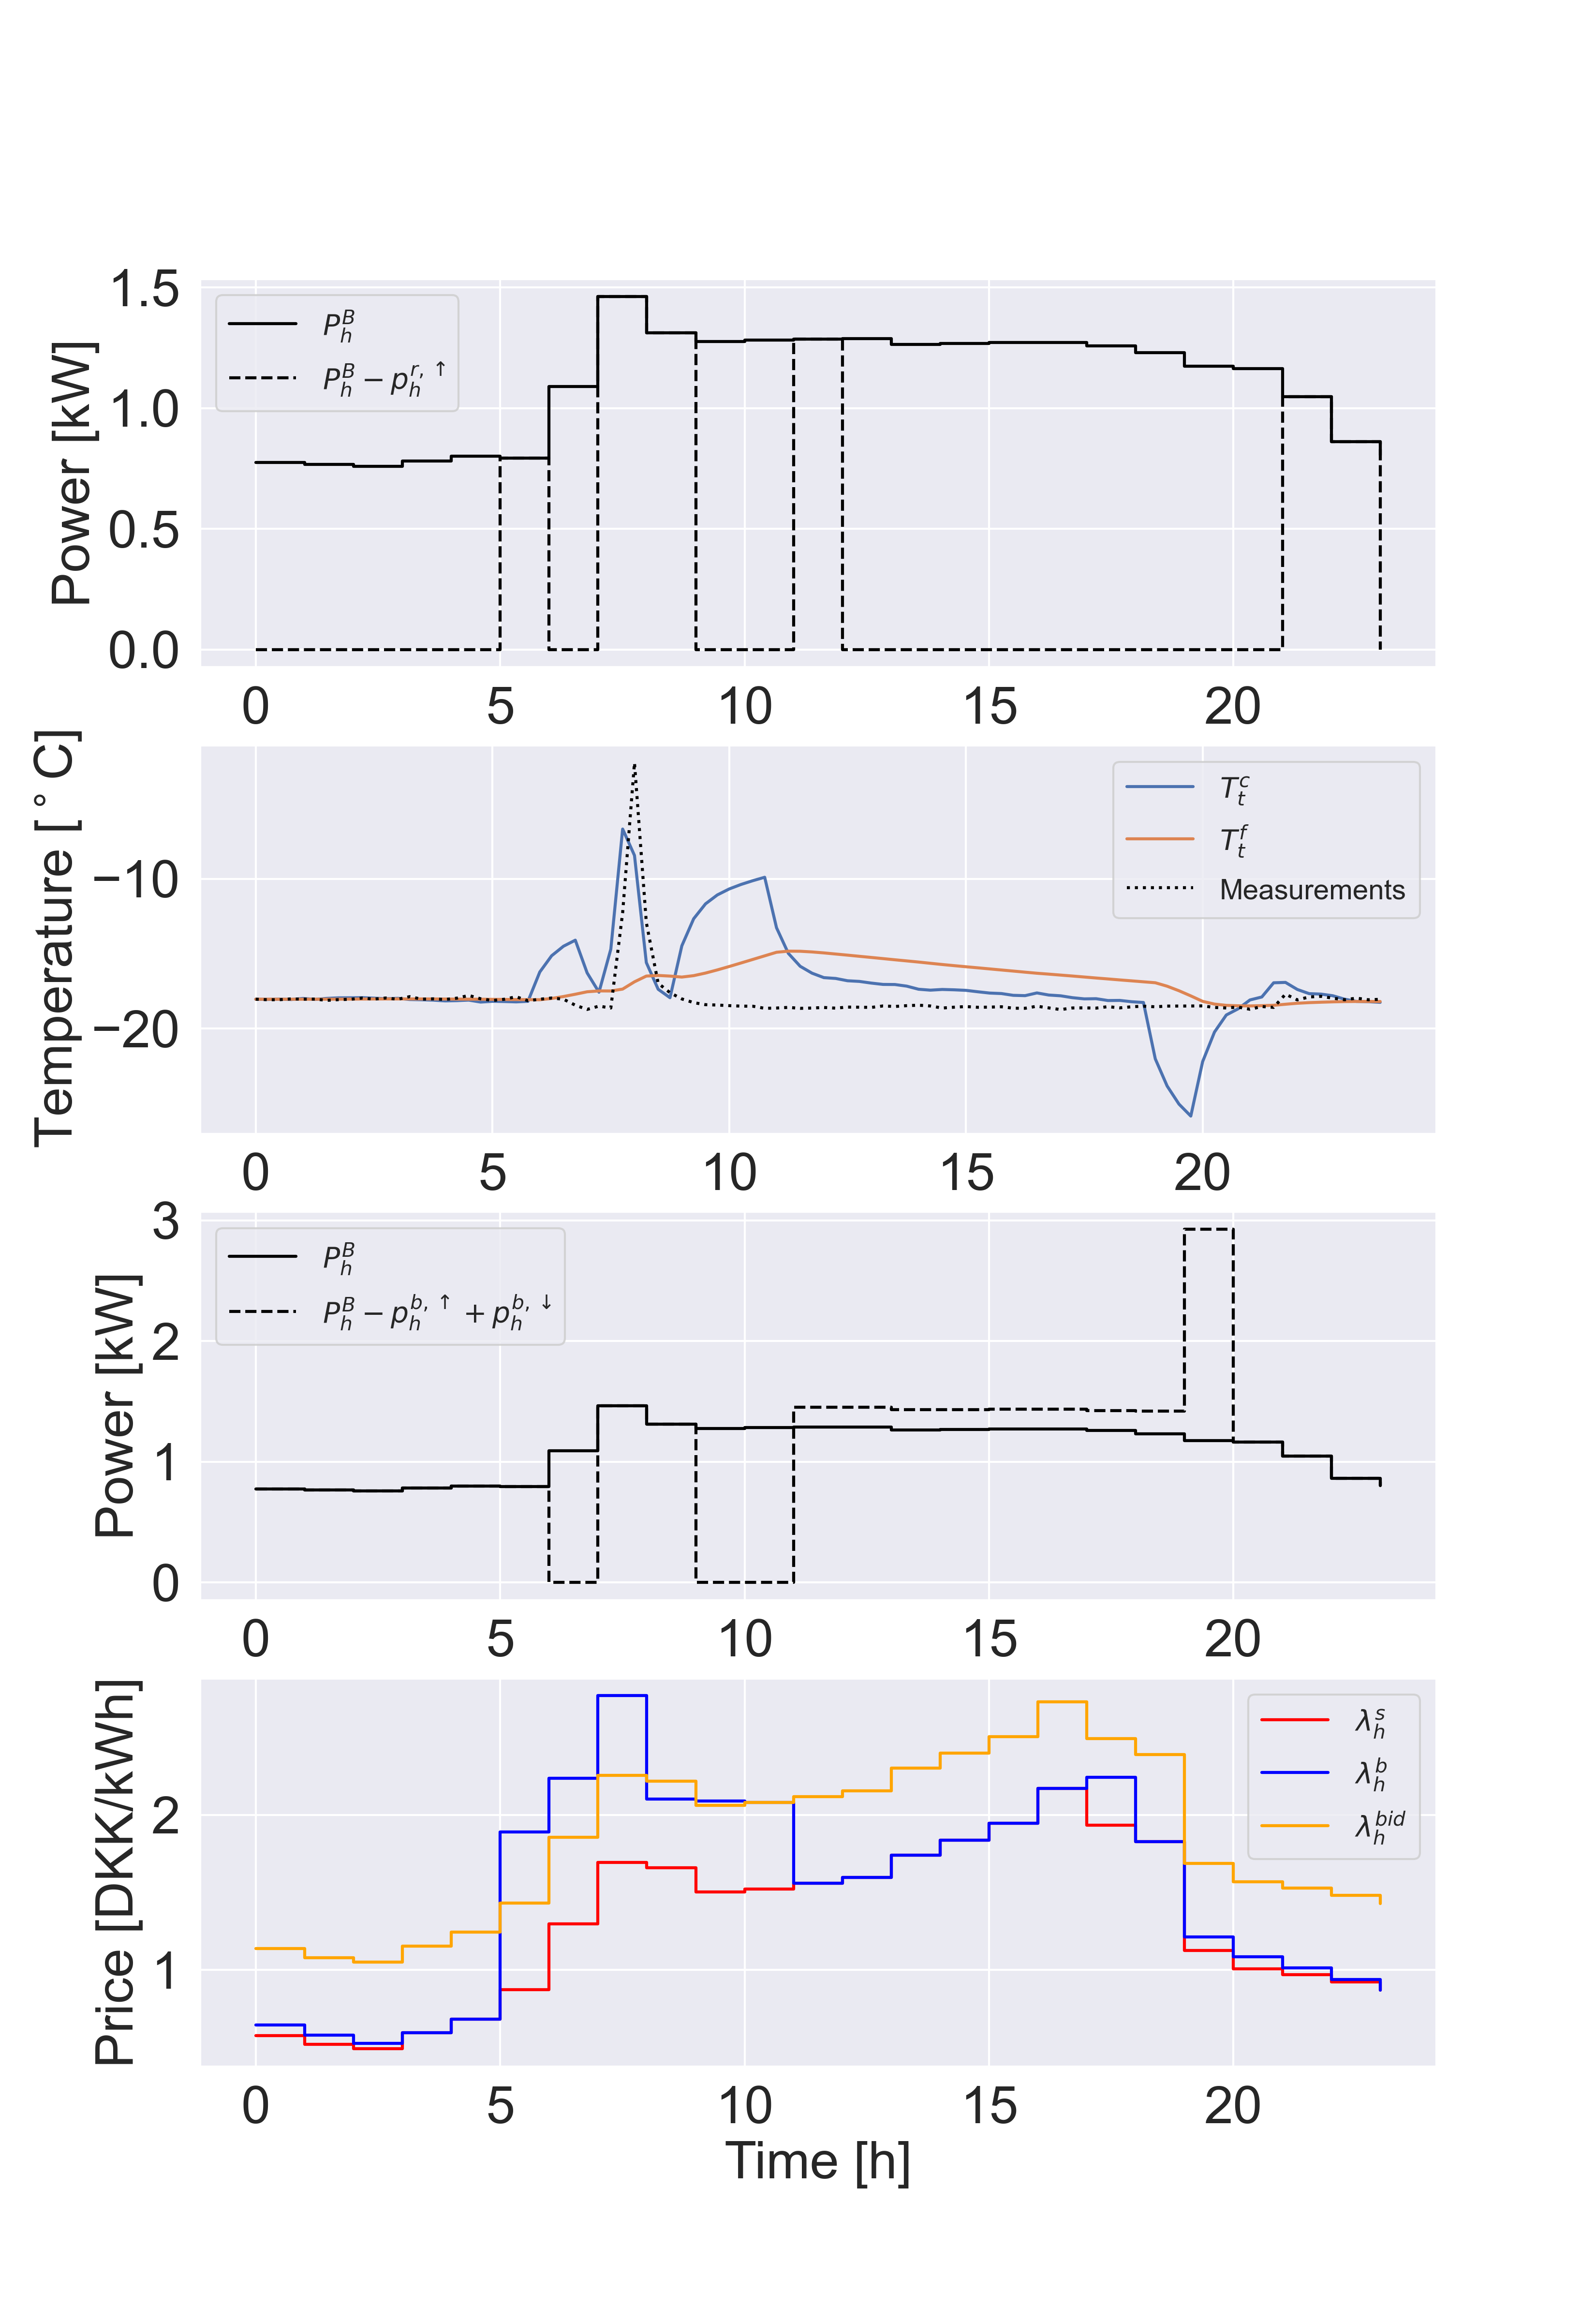
\includegraphics[width=\columnwidth]{../figures/mFRR_single_case.png}
    \caption{Example of mFRR service provision in a representative day (an in-sample scenario). \textbf{Top}: Reservation capacities and baseline power of the freezer. \textbf{Upper middle}: Air and food temperature dynamics. \textbf{Lower middle}: mFRR activation in this specific scenario, i.e., when $\lambda_{h}^{\rm{bid}} \leq \lambda_{h}^{\rm{b}}$, $\lambda_{h}^{\rm{b}} > \lambda_{h}^{\rm{s}}$, and $p^{\rm{r},\uparrow}_{h} > 0$. \textbf{Bottom}: Spot and balancing market price as well as regulating power bids in this specific scenario.}
    \label{fig:fig_second_case}
\end{figure}


\subsection{Technical results}
Fig. \ref{fig:fig_first_case} shows technical results for the case of load shifting in a representative day. For given spot market prices (bottom plot), it is evident that the freezer shifts the load to low-price hours, especially in the later hours of the day (top plot). However, this has a remarkable effect on the air and food temperature with large deviations from the normal set-point (middle plot).

%, load shifting and mFRR are compared for the same day. For load shifting, it can clearly be seen how load is shifted to low-price hours, especially at the end of the day. But it also has a very significant effect on the temperature with large deviations from its normal setpoint. 

Fig. \ref{fig:fig_second_case} presents technical results for the case of mFRR service provision in a representative day, whose spot and balancing market prices are given in the lower plot. The top plot shows the baseline power profile $P^{\text{Base}}_{h}$ and the mFRR reservation $p^{\rm{r}, \uparrow}_{h}$ sold. For a better illustration, we have plotted $P^{\text{Base}}_{h}-p^{\rm{r}, \uparrow}_{h}$, i.e., the power profile of the freezer if the full activation happens during the entire day. The third  plot of Fig. \ref{fig:fig_second_case} shows, for this specific day (as an in-sample scenario), the freezer is activated three times, i.e., in hours 6, 9, and 10. In these three hours, all conditions $\lambda_{h}^{\rm{bid}} \leq \lambda_{h}^{\rm{b}}$, $\lambda_{h}^{\rm{b}} > \lambda_{h}^{\rm{s}}$, and $p^{\rm{r},\uparrow}_{h} > 0$ hold (see the bottom plot). The rebound (down-regulation) happens from hour 11 to 19. Interestingly, the majority of rebound happens in hour 19, because the balancing price is comparatively low. Finally, the second plot shows that the food and air temperature deviations in the freezer due to mFRR service provision are smoother in comparison to the case with load shifting.


%For mFRR, the reservation is almost full for all hours during the day. The activation of reservation occurs when the bid price is lower than the balancing price which in this particular scenario only happens for three hours. The effect on the temperature is therefore much smaller than for load shifting. The model is also able to rebound smartly in hour 19 to avoid high rebound costs.

Our second main observation is as follows: Although the cost saving is higher for load shifting in comparison to mFRR service provision, it is directly proportional to the energy shifted, and therefore, the temperature deviation in the freezer. This is not the case for mFRR due to the mechanism of reservation and activation.



% AS ONE FIGURE
% \begin{figure*}[t]
%     \centering
%     \subfloat[]{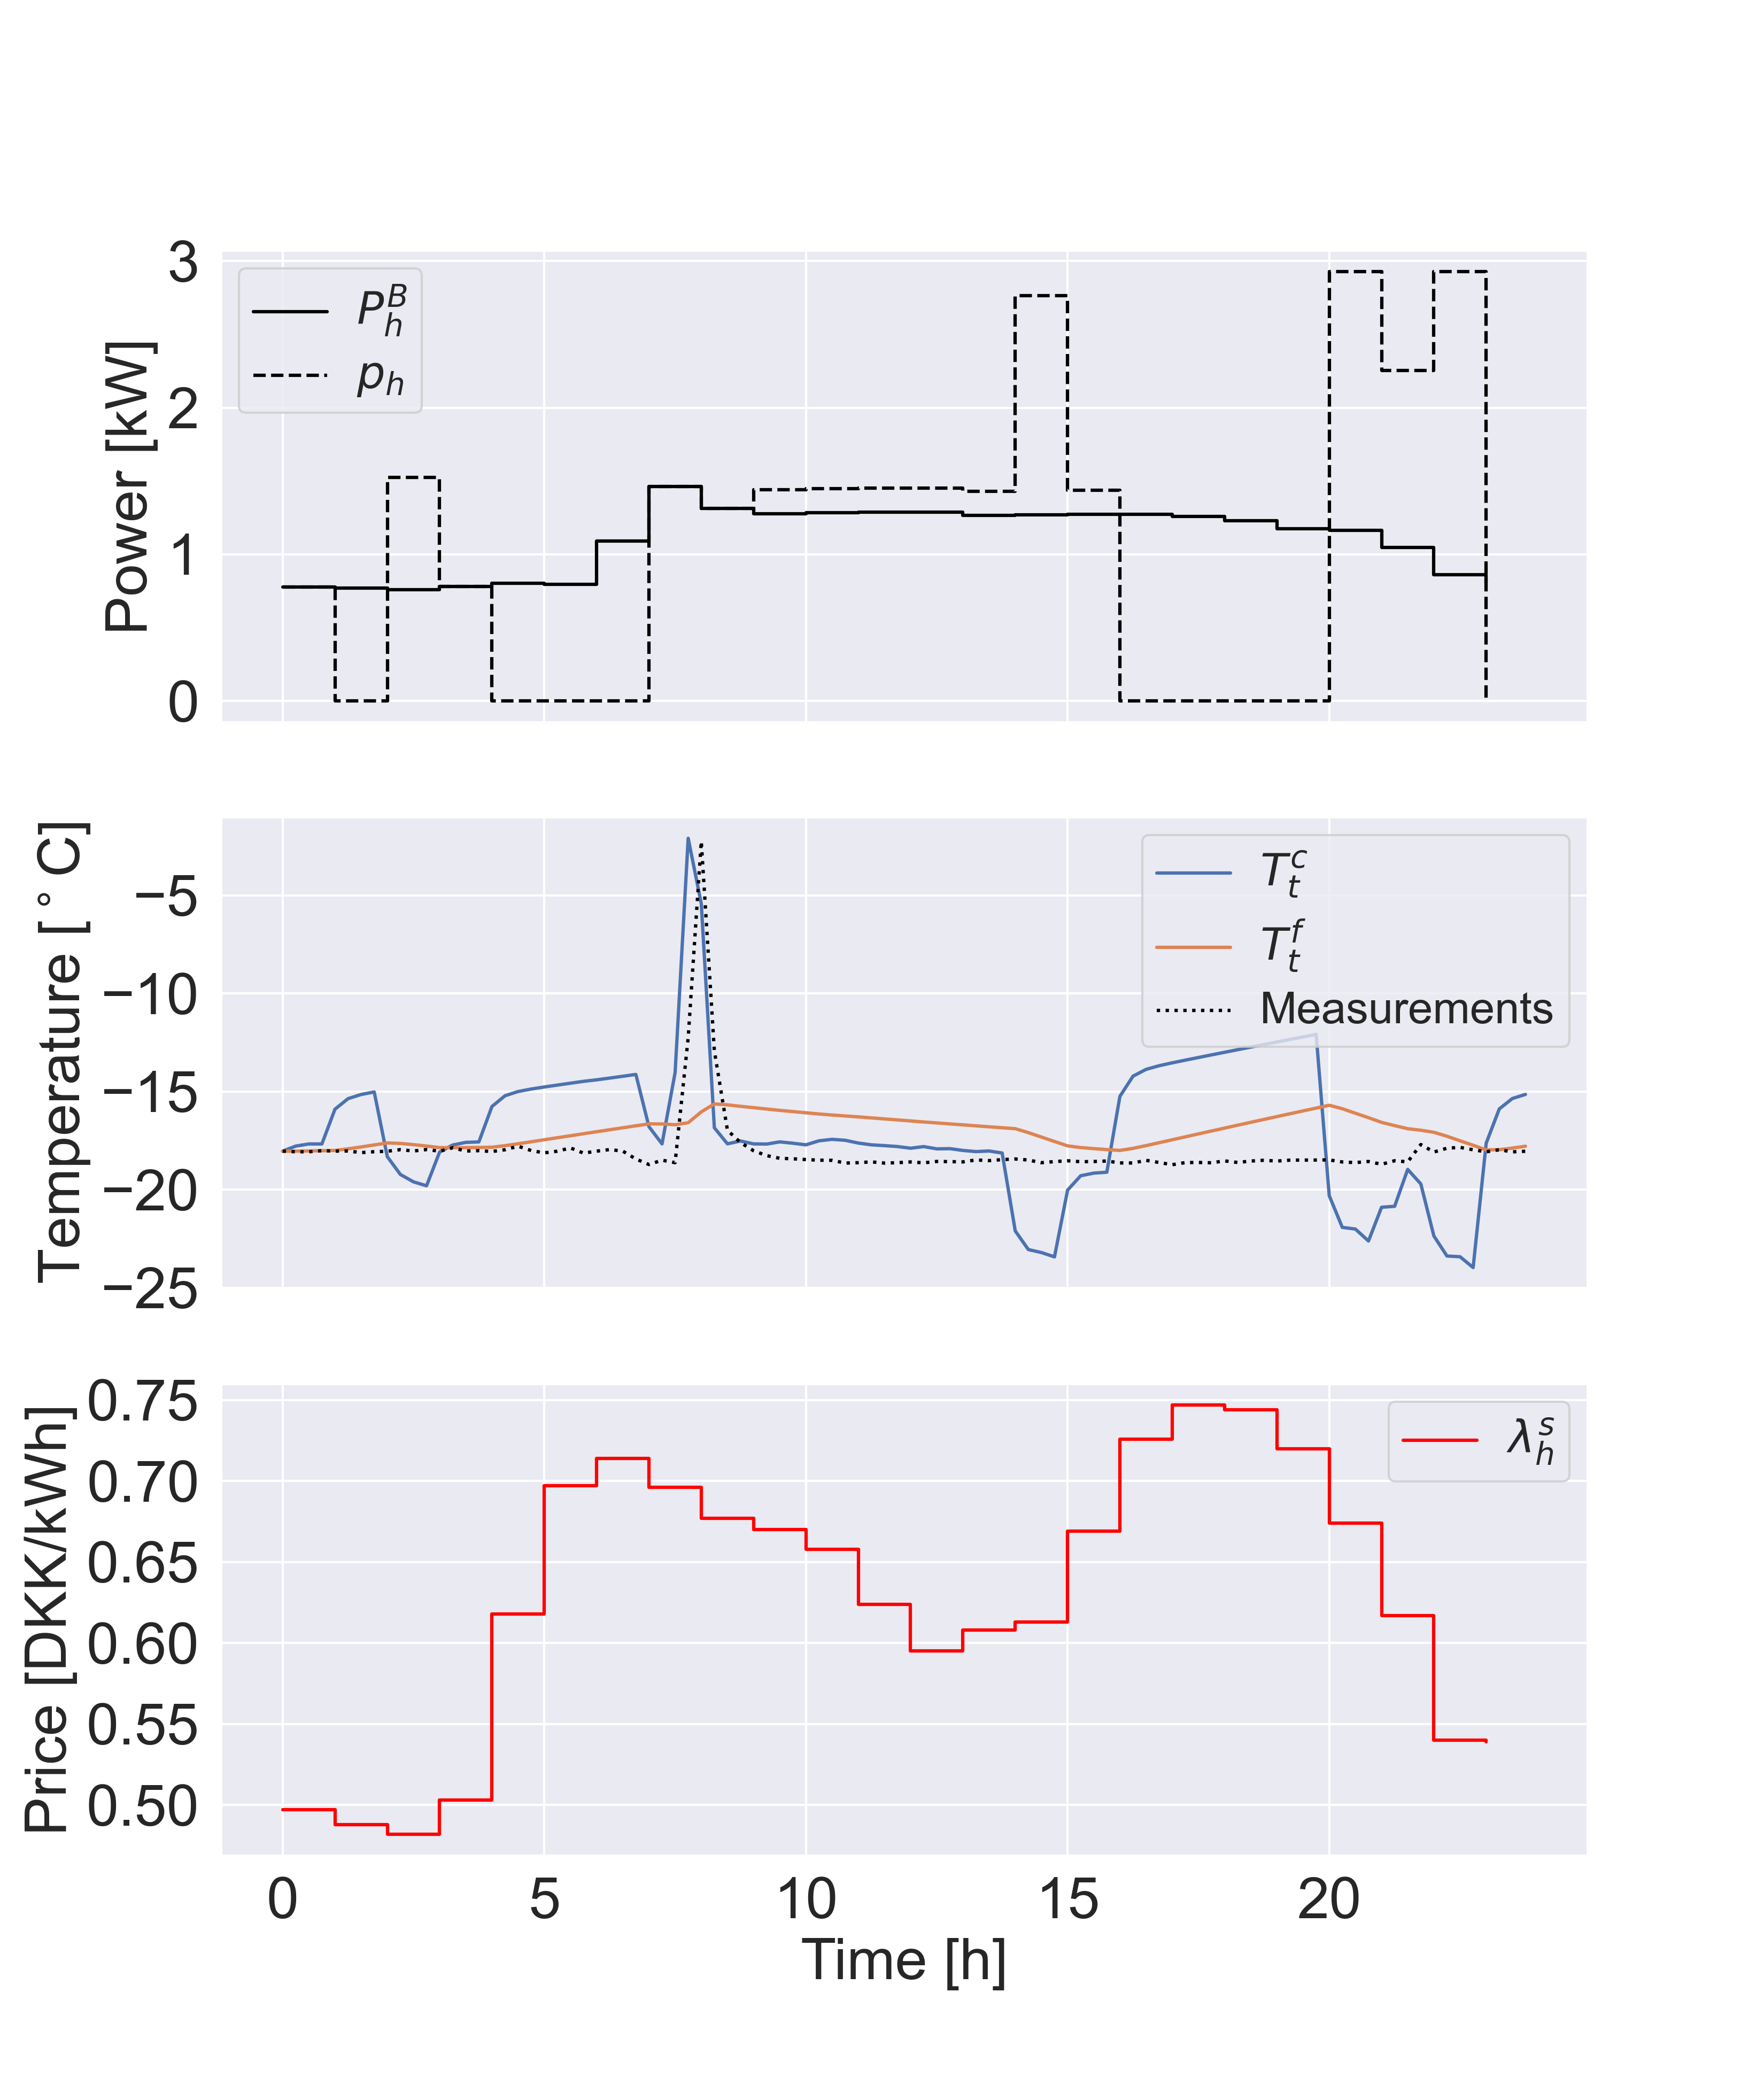
\includegraphics[width=\columnwidth]{../figures/spot_single_case.png}%
%         \label{fig_first_case}}
%     \hfil
%     \subfloat[]{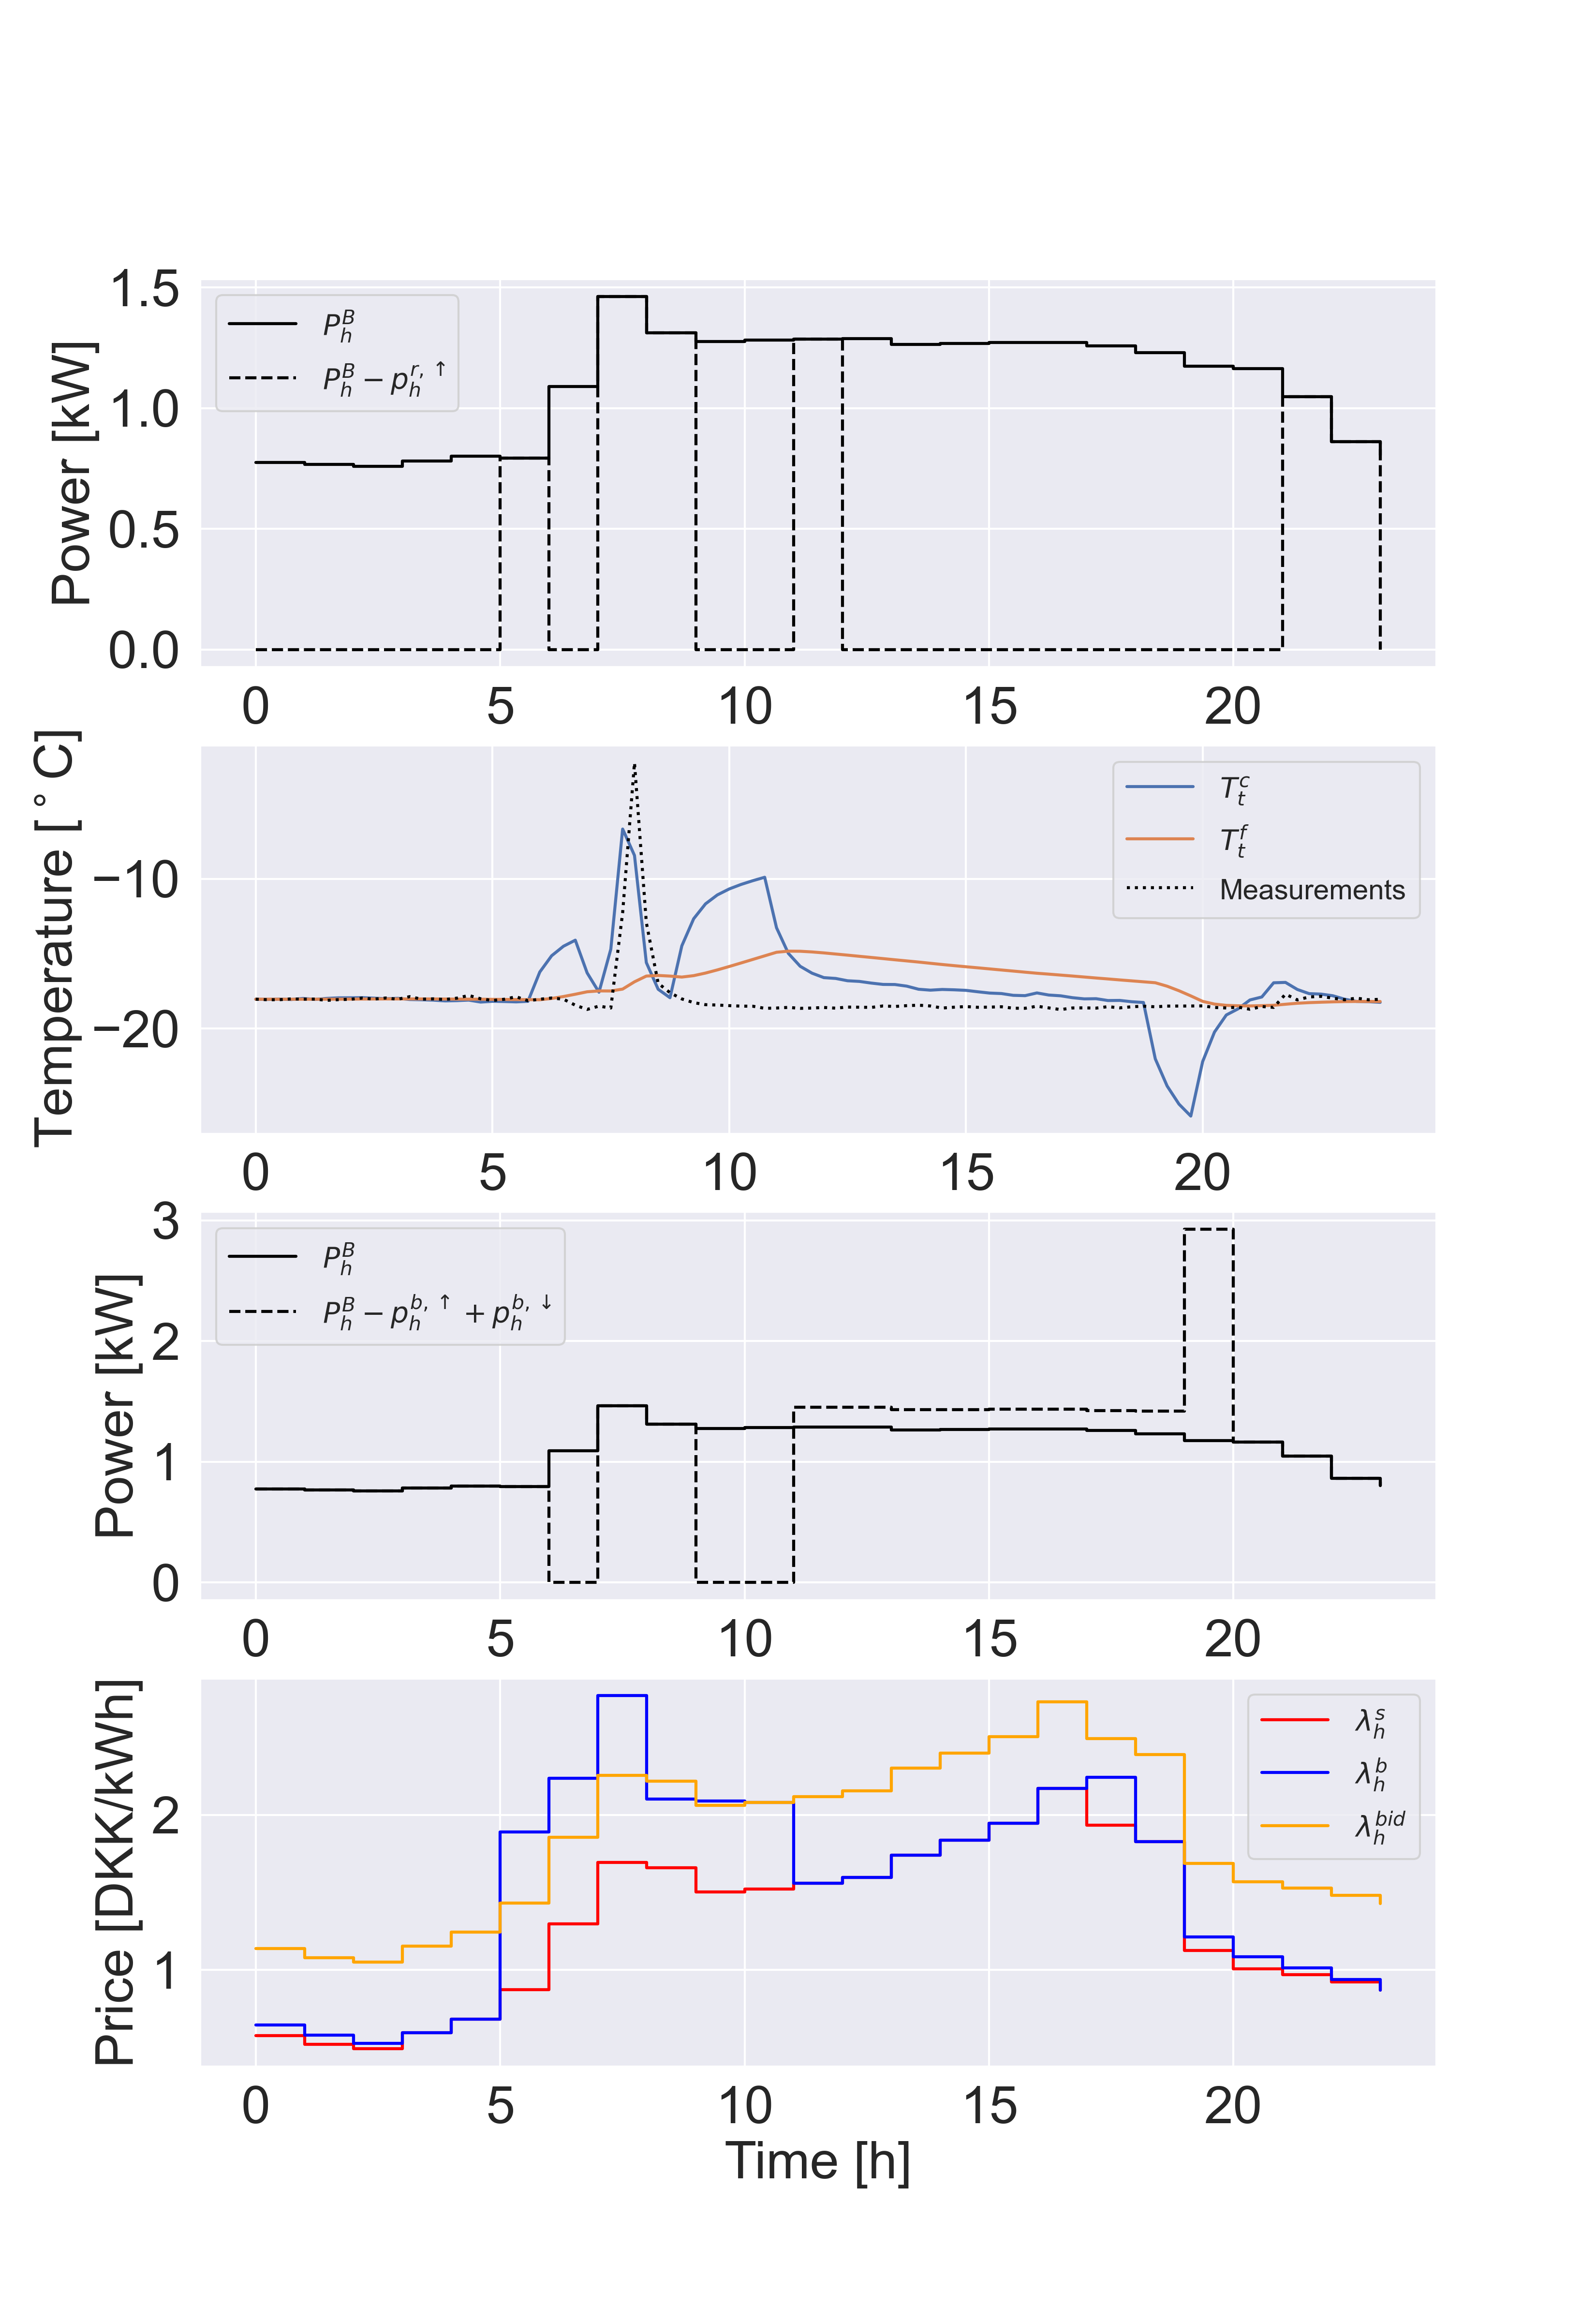
\includegraphics[width=\columnwidth]{../figures/mFRR_single_case.png}%
%         \label{fig_second_case}}
%     \caption{Comparison between load shifting and mFRR in one IS scenario. \textbf{a}: \textbf{Top}: Power profile when load shifting and baseline power of freezer. \textbf{Middle}: Air and food temperature dynamics. \textbf{Bottom}: Spot price in scenario. \textbf{b}: \textbf{Top}: Reservation capacities and baseline power of freezer. \textbf{Upper middle}: Air and food temperature dynamics. \textbf{Lower Middle}: mFRR activations in this scenarios, i.e., when $\lambda_{h}^{bid} \leq \lambda_{h}^{b}$, $\lambda_{h}^{b} > \lambda_{h}^{s}$ and $p^{r,\uparrow}_{h} > 0$. \textbf{Bottom}: Spot price, balancing price, and bid price in scenario.}
%     \label{fig:fig_sim}
% \end{figure*}

% AS TWO FIGURES





%Nevertheless, load shifting seems more appealing for a flexible consumer compared to mFRR from a monetary point of view. This finding illustrates the importance of designing attractive markets for mFRR if demand-side flexibility is to be used more widely, and perhaps also to disincentivize load shifting for flexible consumers as it could lead to system imbalances.


%\subsection{ADMM}
%Figure \ref{fig:admm_vs_normal_solution} shows the ADMM convergence to the optimal solution for five scenarios for different step sizes. For most step sizes, it converges quickly but never quite reaches the optimal solution. This is mainly because the algorithm has to achieve consensus on three variables, $p_{h,\omega}^{r,\uparrow}$, $\alpha_{\omega}$, and $\beta_{\omega}$. Experiments showed that it was converging much closer to the optimal solution when removing $\alpha_{\omega}$, and $\beta_{\omega}$.

%A large step size emphasizes the need to reach consensus whereas a small step size prioritizes the objective function in (\ref{P1:eq1}). Here, it seems a step size of $\gamma \geq 1$ is more stable and converges quickly.

%\begin{figure}[!t]
%    \centering
%    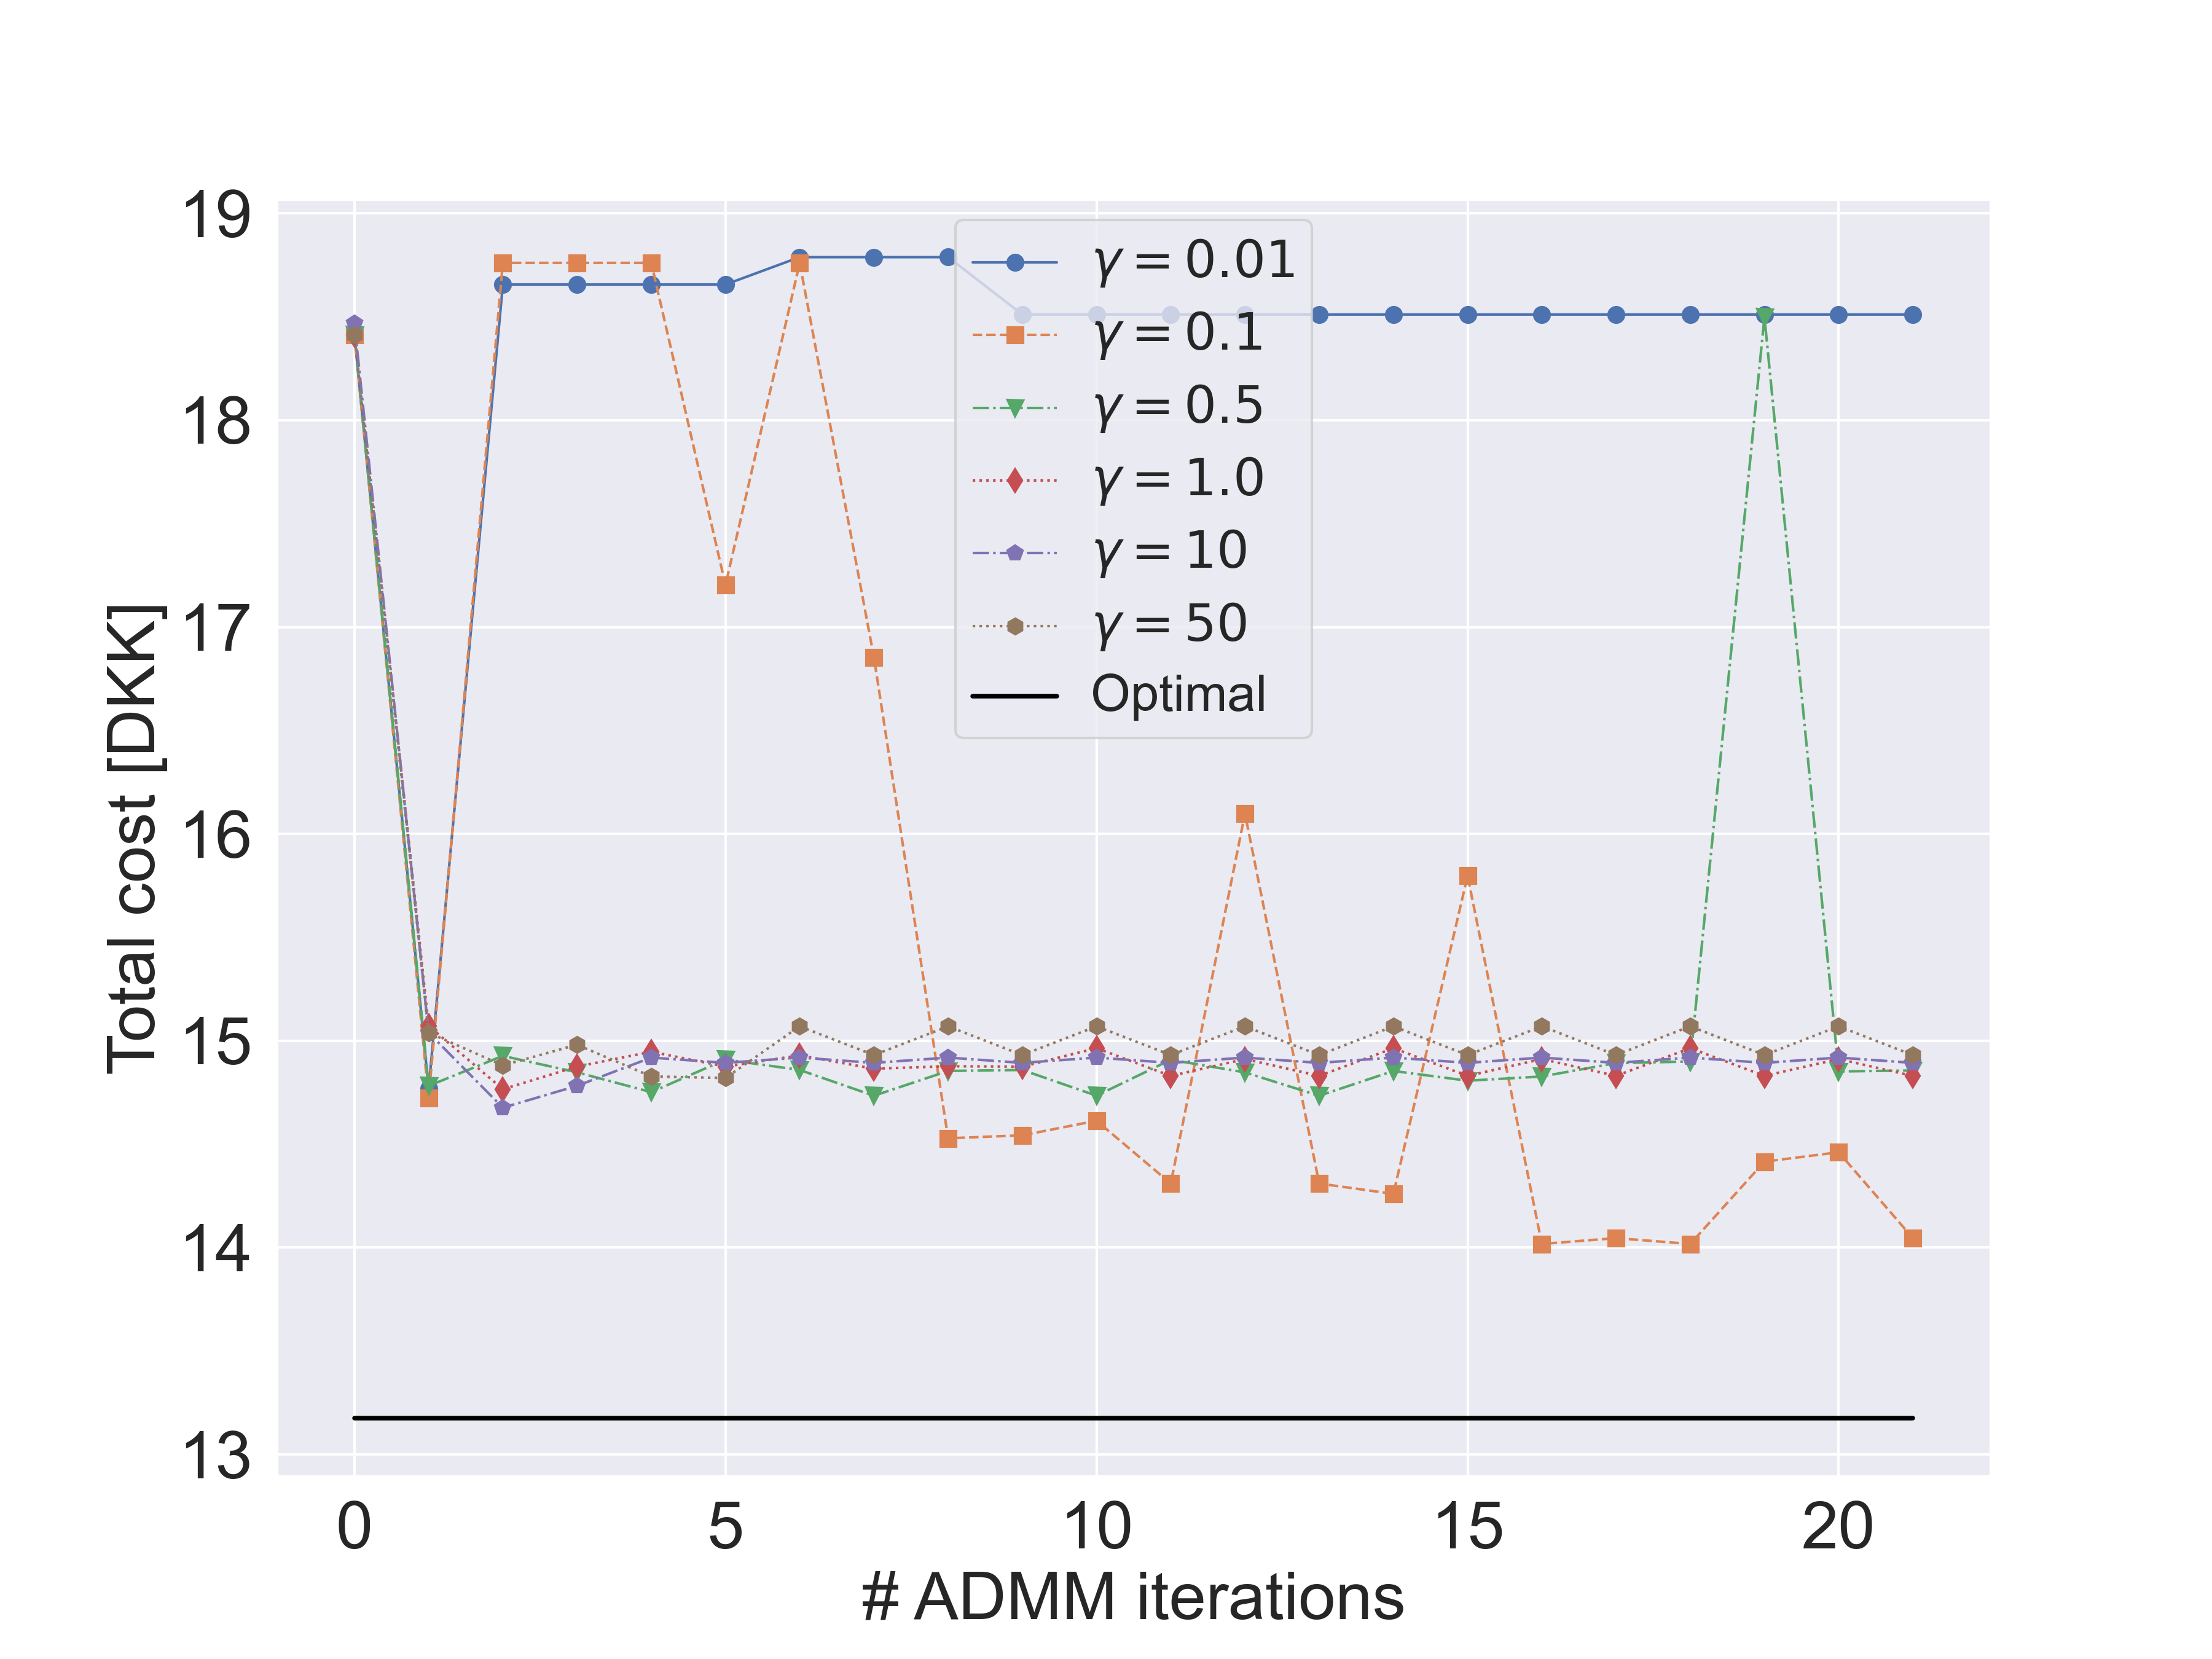
\includegraphics[width=\columnwidth]{../figures/admm_vs_normal_solution.png}
%    \caption{ADMM solution versus the optimal solution for five scenarios for different step sizes in the ADMM algorithm.}
%    \label{fig:admm_vs_normal_solution}
%\end{figure}

%Figure \ref{fig:admm_nb_scenarios_effect} shows the effect of including more scenarios in Problem (\ref{P1:compact_model}) using ADMM to solve it. For IS, good solutions are already obtained with 5-10 scenarios, and the same applies for OOS although it seems using 250 scenarios also performs well.

%The plot highlights the importance of choosing representative scenarios, especially balancing prices as they determine how much activation is needed, and therefore the bid policy.

%\begin{figure}[!t]
%    \centering
%    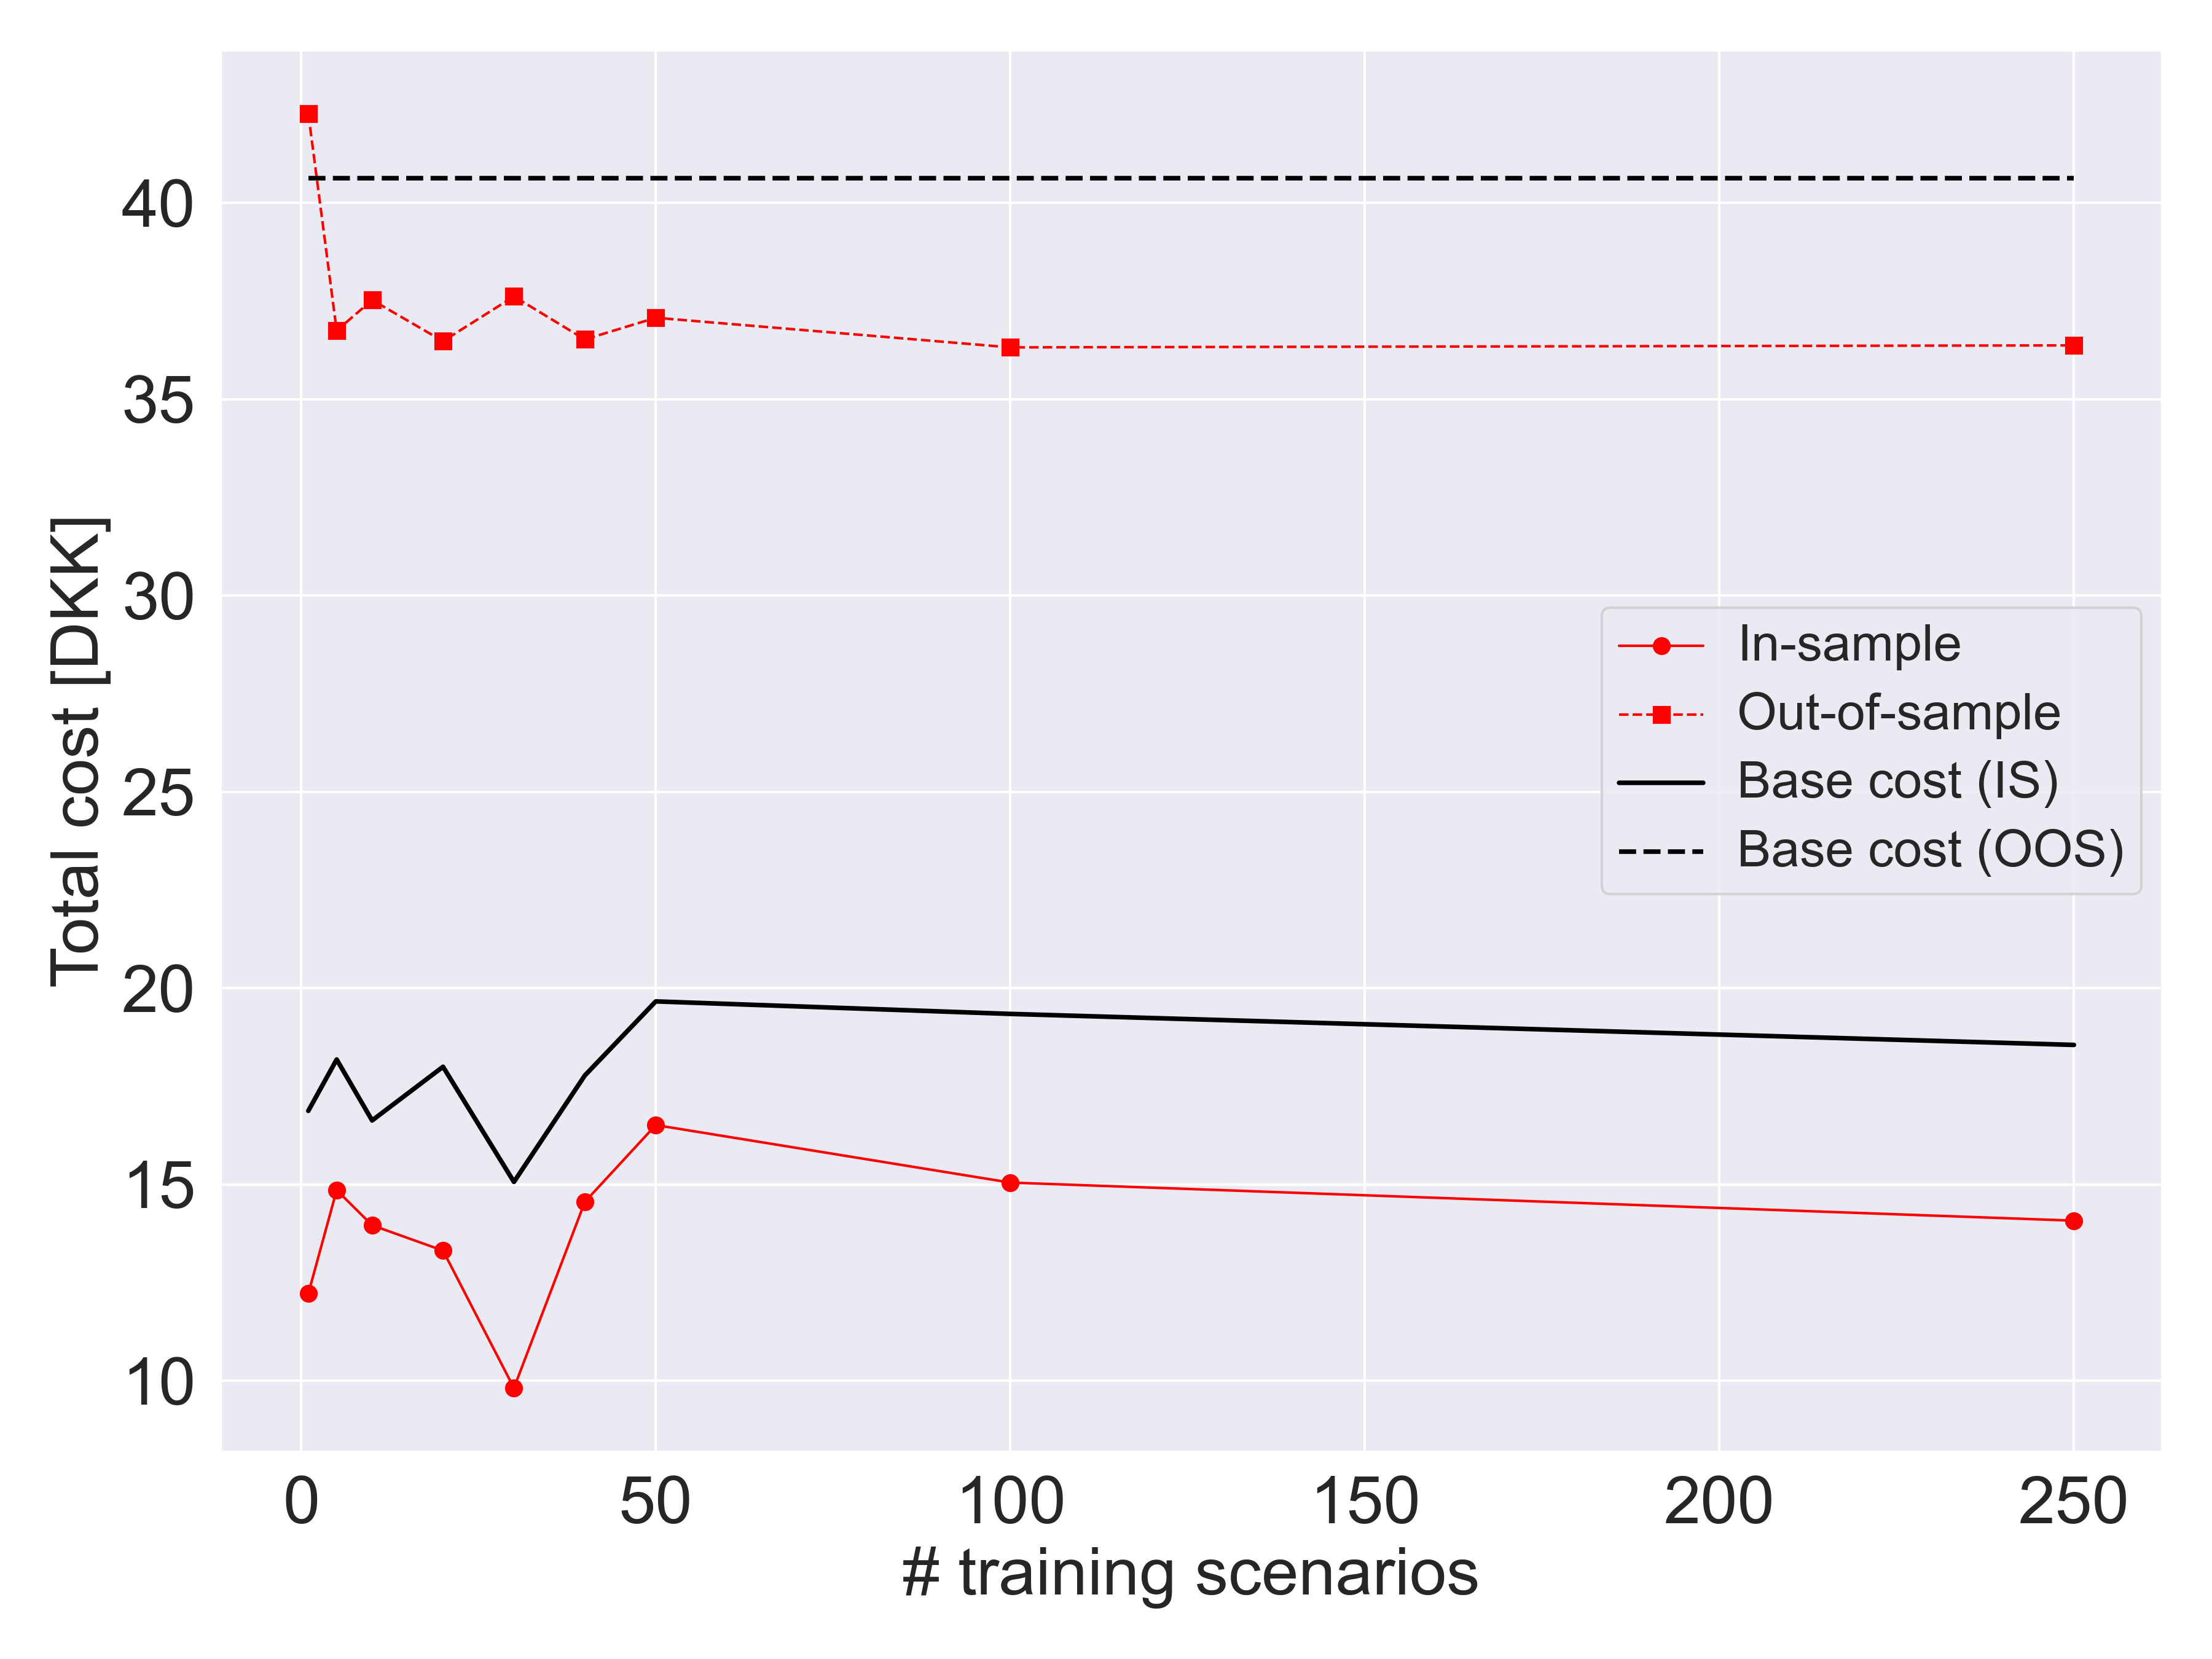
\includegraphics[width=\columnwidth]{../figures/admm_nb_scenarios_effect.png}
%    \caption{Effect of number of IS scenarios on OOS performance for ADMM. Both are compared to the baseline costs of the freezer.}
%    \label{fig:admm_nb_scenarios_effect}
%\end{figure}

% \subsection{Lookback}

% TODO: create plot of effect of lookback parameter.
